\chapter{Signal Processing}
\begin{item}
\item[white noise]White noise is the noise signal whose power spectrum is flat i.e. will have almost constant integrated power at different frequency bands of same duration (bandwidth). White noise is made of almost all the frequencies and will have constant power at all these frequencies; hence it is also analogous to white light emitting all the frequencies in the same proportion. The figure describes spectrum of white noise.
\begin{figure}
  \centering
  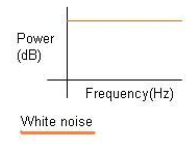
\includegraphics[scale=0.45]{images/I/wn.png}
  \caption{White noise}\label{fig:wn}
\end{figure}

\item[coloured noise]Colored noise will have different integrated power at different frequency bands of same duration. Depending upon whether it is gray, pink, blue or brown color it will have different power spectrum. Based on this power concentration varies at different frequencies. The figure describes spectrum of colored noise(example-Pink noise).
\begin{figure}
  \centering
  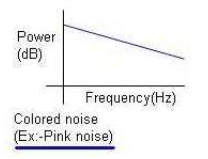
\includegraphics[scale=0.45]{images/I/cn.png}
  \caption{Coloured noise}\label{fig:cn}
\end{figure}

\end{item}

